\documentclass{article}
\usepackage[utf8]{inputenc}
\usepackage{graphicx}
\usepackage{geometry}
\usepackage{amsmath}
\usepackage{amsfonts}
\usepackage{float}
\usepackage{caption}
\usepackage{subcaption}
\usepackage{enumitem}

\geometry{left=25mm, top=25mm, right=25mm, bottom=25mm}

\title{PHY407 Lab 11}
\author{Pierino Zindel (1002429703) and Hayden Johnson (1002103537)}
\date{November 30, 2018}

\begin{document}

\maketitle

\noindent \textbf{Distribution of work:} Questions 1 and 2 were completed by Hayden. Questions 3 and 4 were completed by Pierino.

\section{A First Monte Carlo Simulation}

\subsection{Part a)}

We seek to create plots of the energy as a function of time for the simulated ideal gas, as well as the frequency distribution of the energy of individual particles once the system reaches equlibrium, in the case $k_BT=10$ for the simulation of an ideal gas provided.

We were able to achieve this with effectively no modifications to the code provided. The graphs produced are provided below in figures \ref{fig:q1a_energy} and \ref{fig:q1a_hist}.

\begin{figure}[H]
	\centering
	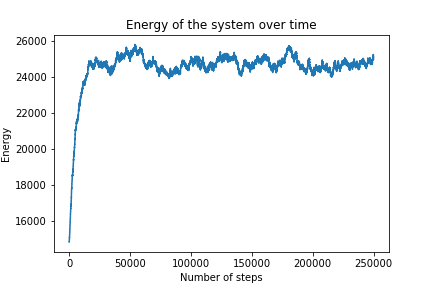
\includegraphics[width=0.7\textwidth]{../images/q1a_energy.png}
	\caption{Plot of the energy of the system over 250000 steps of the process of randomly increasing the states of random particles depending on the energy and temperature of the system.}
	\label{fig:q1a_energy}
\end{figure}

\begin{figure}[H]
	\centering
	\begin{minipage}{0.49\linewidth}
		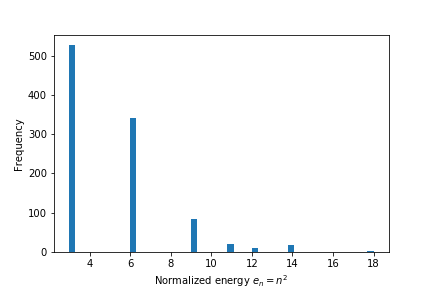
\includegraphics[width=\linewidth]{../images/q1a_energy_hist.png}
	\end{minipage}
		\begin{minipage}{0.49\linewidth}
		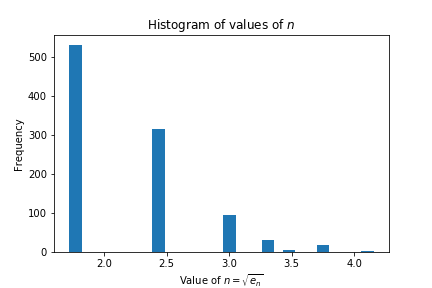
\includegraphics[width=\linewidth]{../images/q1a_n_hist.png}
	\end{minipage}
	\caption{Histograms of the distribution of values of the normalized energy $e_n = n^2$ (left) and the value of $n$ (right) for the system after 250,000 steps, when it is in equilibrium.}
	\label{fig:q1a_hist}
\end{figure}

\subsection{Part b)}

We seek to calculate the value of the total energy at equilibrium, and the average value of the quantum number $n$, for the system at various temperatures.

In order to achieve this, we adapted the code from part a) to iterate over the different temperatures desired, and run the Monte Carlo energy calculating scheme for each. In order to determine how long to run the simulation for at each temperature, we used a condition which would, at every 200,000th step, calculate the average energy across the most recent 200,000 steps and compare it to that of the previous set of 200,000 steps. Once the average energy of the more recent set of 200,000 steps is less than or equal to that of the previous set, we conclude that the system must have reached equilibrium, and stop iterating. The value of 200,000 was chosen from a combination of visual inspection of the size of the fluctuations in the energy and a component of trial and error.

\begin{figure}[H]
	\centering
	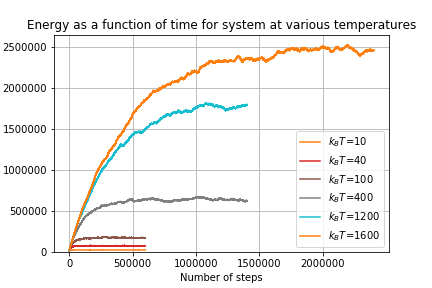
\includegraphics[width=0.8\textwidth]{../images/q1b_energies.png}
	\caption{Energy as a function of time for six different temperatures of the system, plotted until they reach equilibrium.}
	\label{fig:q1b_energies}
\end{figure}

\begin{figure}[H]
	\centering
	\begin{minipage}{0.49\linewidth}
		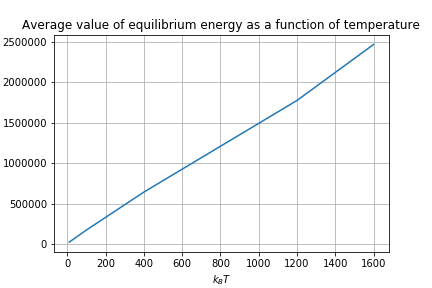
\includegraphics[width=\linewidth]{../images/q1b_av_energy.png}
		\caption{Equilibrium energy as a function of system temperature for the range of temperatures tested.}
		\label{fig:q1b_av_energy}
	\end{minipage}
	\begin{minipage}{0.49\linewidth}
		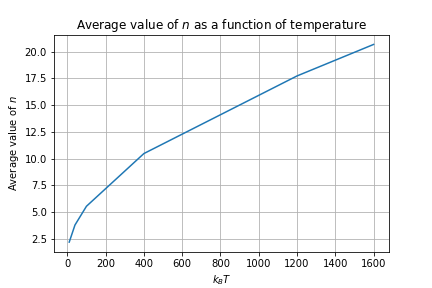
\includegraphics[width=\linewidth]{../images/q1b_av_n.png}
		\caption{Average value of $n$ as a function of system temperature for the range of temperatures tested.}
		\label{fig:q1b_av_n}
	\end{minipage}
\end{figure}

For each temperature, we computed the average value of $n$ using equation 5 from the handout, as well as stored the average value of the energy once the system reached equilibrium; these are plotted in figures \ref{fig:q1b_av_n} and \ref{fig:q1b_av_energy}, respectively. From the slope of the graph in figure \ref{fig:q1b_av_energy}, we calculate that the value of $\Delta E / \Delta T$ over the range of temperatures tested is approximately:
\begin{equation}
	\frac{\Delta E}{\Delta T} \approx 1535
\end{equation}

\section{Ising Model}

\begin{figure}[H]
	\begin{minipage}{0.49\linewidth}
		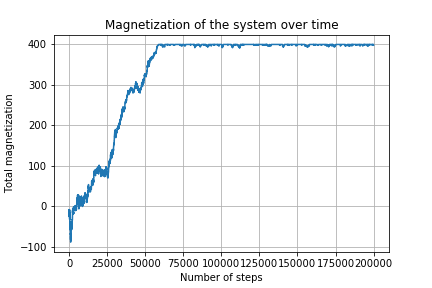
\includegraphics[width=\linewidth]{../images/q2_magnetization_pos.png}
	\end{minipage}
	\begin{minipage}{0.49\linewidth}
		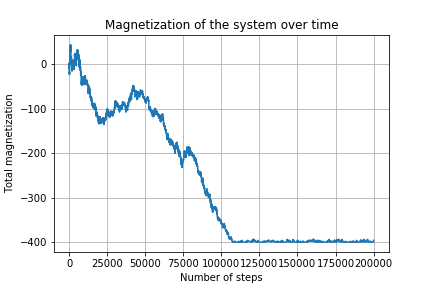
\includegraphics[width=\linewidth]{../images/q2_magnetization_neg.png}
	\end{minipage}
	\caption{Plots of total magnetization of the system over time. The system can spontaneously drift to either a completely positive (left) or completely negative (right) magnetization, with an equal chance of either occurring, based on the initial conditions and early random dipole flips.}
	\label{fig:q2_magnetization}
\end{figure}

\section{Simulated Annealing Warm-up}

\section{Dimer Covering Problem}


\end{document}